\section{Methodology}

In this work, we implement two benchmark models, and four few-shot machine learning architectures. Molecules are represented using graph objects, which are processed using graph convolutional networks (GCNs). IterRefLSTMs are used to enrich the resulting embeddings in latent space. The following sections go into the implementations in more detail.

\subsection{Datasets}

In this work, we make use of the following three datasets;

\textit{Tox21} \cite{huang2016tox21challenge}. Mainly used for lead optimisation, containing toxicity data for 12 targets \citep{tox21}. The dataset was obtained from the DeepChem AWS bucket\footnote{Accessed from: deepchemdata.s3-us-west-1.amazonaws.com/datasets/tox21.csv.gz. Last Accessed: 08/11/2021} in CSV format. The NR-AR, NR-AR-LBD, NR-AhR, NR-Aromatase, NR-ER, NR-ER-LBD, NR-PPAR-gamma, SR-ARE, SR-ATAD5 targets are reserved for training, and the remaining SR-HSE, SR-MMP, SR-p53 targets for testing.
\textit{Maximum Unbiased Validation (MUV)} \citep{rohrer2009maximum}. Based on PubChem BioAssays, used for validating virtual screening techniques against 17 different targets \citep{rohrer2009maximum}. The dataset was obtained from the DeepChem AWS bucket\footnote{Accessed from: deepchemdata.s3-us-west-1.amazonaws.com/datasets/muv.csv.gz. Last Accessed: 08/11/2021} in CSV format. A total of 12 targets (MUV-466 - MUV-810) are reserved for training, while MUV-832, MUV-846, MUV-852, MUV-858, and MUV-859 are reserved for testing.
\textit{Directory of Useful Decoys (Enhanced) (DUD-E)} \cite{mysinger2012directory}. Used for benchmarking virtual screening techniques by introducing a number of active compounds against specific targets. For each active, a number of \textit{decoys} with similar physical properties, but different topologies, are made available. For this research study, we made use of the GPCR subset of the DUD-E dataset \citep{mysinger2012directory}. The data was obtained directly from the DUD-E website.\footnote{Accessed from: http://dude.docking.org/subsets. Last Accessed: 08/11/2021} The AA2AR, DRD3, and ADRB1 are used for training. Two targets are reserved for testing, in which ADRB2 contains decoys that are auto-generated against a set of known active ligands, while for the CXCR4 target these are hand-picked. 

\begin{table}[h]
	\centering
	\caption{Number of actives and inactives/decoys across all targets in the datasets used. Figures in parentheses show the percentage of the total compounds in the dataset.}
	\begin{tabular}{@{}crr@{}}
		\hline
		Dataset & Actives & Inactives/Decoys \\
		\hline
		Tox21 & 4,149 (7.04\%) & 54,746 (92.96\%) \\
		\hline
		MUV & 347 (0.20\%) & 175,990 (99.80\%) \\
		\hline
		DUD-E (GPCR) & 1,249 (1.45\%) & 84,856 (98.55\%) \\
	\end{tabular}
	\label{table:datasetimbalance}
\end{table}

\subsection{Molecular Representations}

We first create a molecular graph from the SMILES string using RDKit, an open-source toolkit for cheminformatics. Standardisation of compounds according to a set of well-defined and consistent rules and conventions is of utmost importance to maintain uniformity and integrity across the data being used. \citet{bento2020open} present an open source chemical structure curation pipeline based on RDKit for validating and standardising chemical structures, which follow FDA/IUPAC guidelines \citep{brecher2006graphical, food2007substance}. Their work is available in the ChEMBL Structure Pipeline package \cite{bento2020open} and is used to standardise the molecules in our pipeline. We then create one-hot encoded features for the atoms in each molecule, namely, atom type, atomic number, atom degree, explicit valence, hybridisation, formal charge, number of radical electrons, and aromaticity. Self loops are added to every node in the generated graph, so aggregation functions during message passing consider the features of the node itself. The order of the atoms follows the canonical order of the atoms assigned through RDKit. We make use of the DGL LifeSci \cite{dgllife} library to create the graph objects and subsequently process them using the DGL library \cite{wang2019dgl}.


\subsection{Machine Learning Models}

Before processing the molecular graph, we first learn an embedding using graph neural networks. Four different architectures, including Siamese, Matching, Prototypical and Relation Networks, process the learned graph embeddings to train our meta-learner. IterRefLSTMs are utilised to refine the latent space embeddings.
\begin{figure}[h]
	\centering
	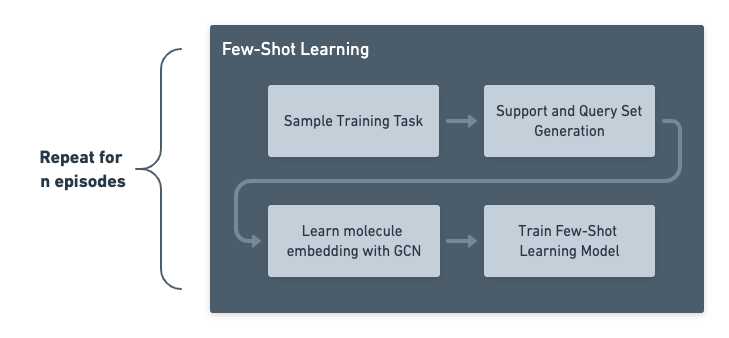
\includegraphics[width=0.9\linewidth]{img/episodic-learning.png}
	\caption{Episodic learning schematic}
	\label{fig:episodiclearning}
\end{figure}

\begin{figure*}
	\centering
	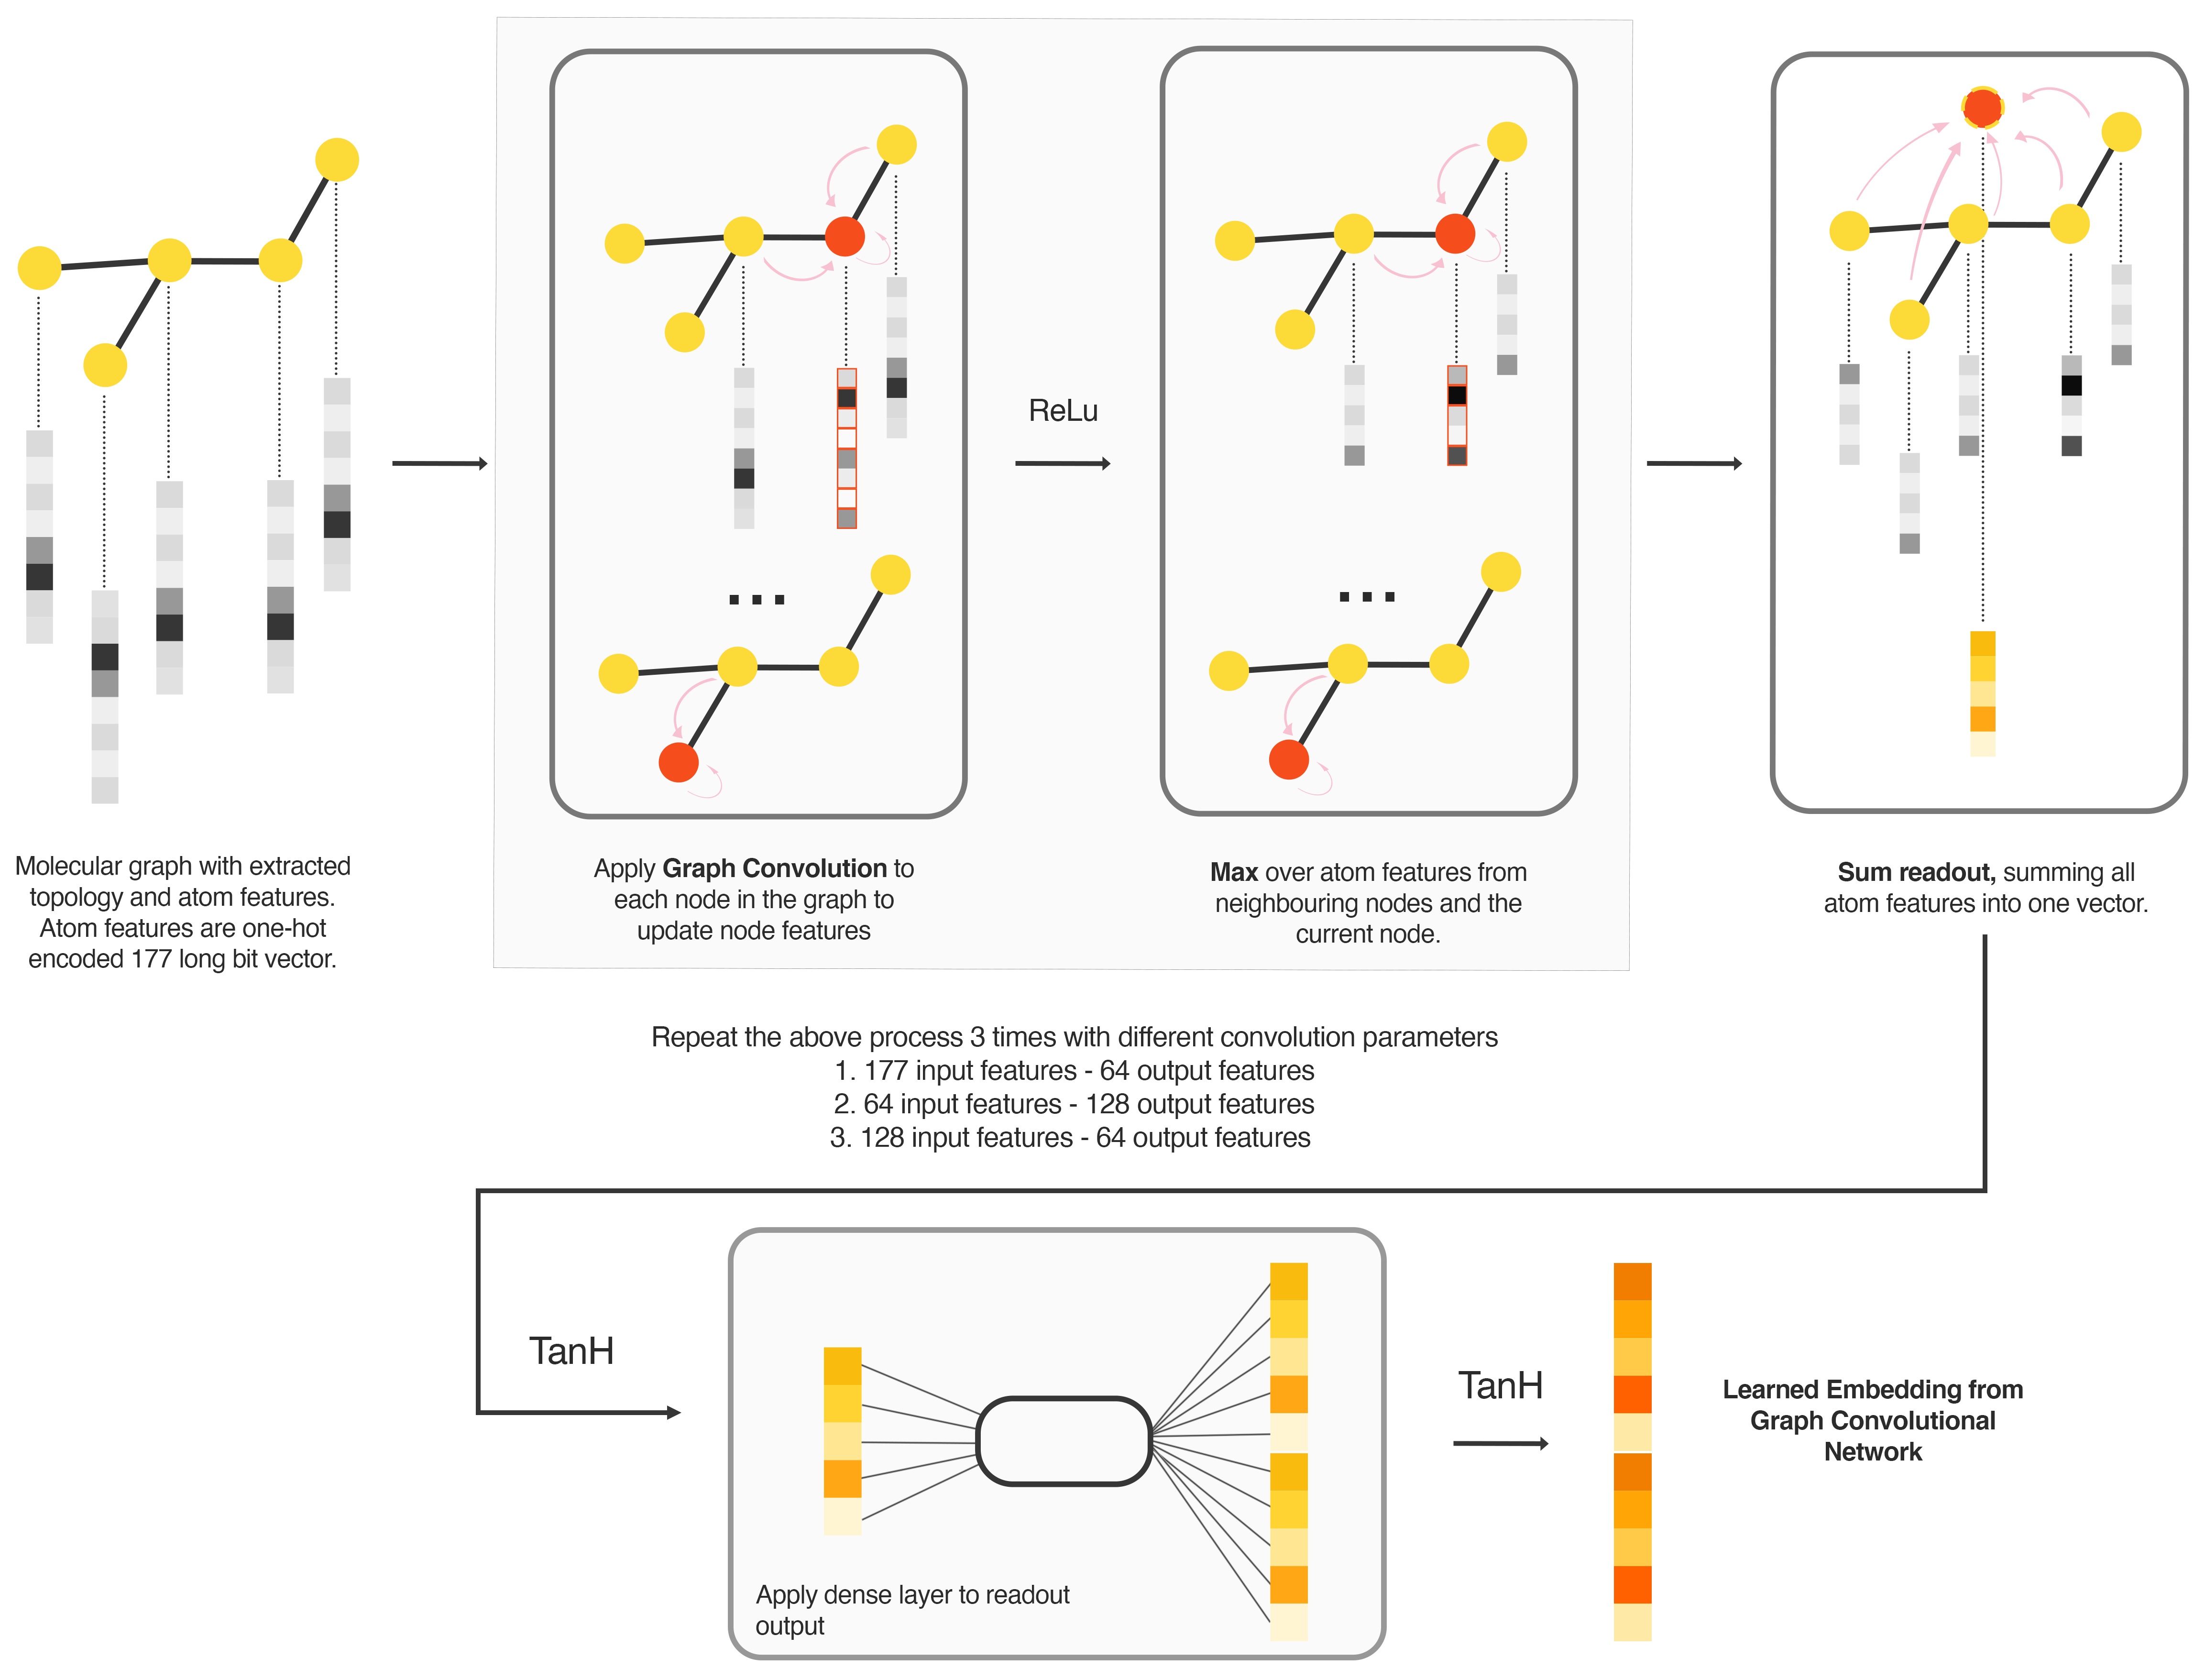
\includegraphics[width=0.75\textwidth]{img/DVGCNArchi.png}
	\caption{Learning an embedding through a Graph Convolutional Network (GCN). The molecule, represented as a graph object with nodes, edges, and atom features, is processed using graph convolutions. A max message-passing function over the current and neighbouring nodes follows each convolution layer. After this process, a sum readout aggregates all atom features into one vector. A TanH function activates this vector, and a dense linear layer processes the output vector. A non-linear TanH function activates this vector to yield the final learned molecular embedding.}
	\label{fig:dvgcnarchi}
\end{figure*}

\subsubsection{Graph Convolutional Networks}

Graph convolutional networks (GCNs) are used to learn embeddings for the support and query molecules in latent space. Figure~\ref{fig:dvgcnarchi} illustrates the GCN pipeline to learn a molecular embedding. In our study, we make use of the convolutional operator from \citet{kipf2016semi} to process graphs and learn the molecular embeddings. The convolutional layer can be mathematically defined through Equation~\ref{gcnequation2}. $h_j$ is the feature set of the node, $N_i$ is the set of neighbouring nodes $i$, $b$ is the learnable bias, and $c_ji$ is the product of the square root of node degrees. From a message-passing perspective, this can be summarised into the following steps for every node feature space $u$;

\begin{equation}
	\label{gcnequation2}
	h_i^{(l+1)} = \sigma(b^{(l)} + \sum_{j\in\mathcal{N}(i)}\frac{1}{c_{ji}}h_j^{(l)}W^{(l)})
\end{equation}

\begin{enumerate}
	\item Aggregating the neighbouring representations $h_v$, producing an intermediate representation $\hat{h}_u$.
	\item Transforming $\hat{h}_u$ through a linear projection and a non-linearity function such that $h_u = f(W_u \hat{h}_u)$ \citep{kipf2016semi}.
\end{enumerate}

Three convolutional layers are present in our architecture, after which a maximum function aggregating the node features with the maximum value of the neighbours and the node itself is applied. We highlight that this is not a coarsening operation, as the number of nodes remain the same. Finally, we apply a global pooling layer (readout), in which we sum over the node features of the graph (see Equation~\ref{gcnequationsum}). A linear transformation is applied to the output from the read-out layer, followed by a non-linear activation function, for which we use a hyperbolic tangent function (TanH), outputting the final molecule embedding.

\begin{equation}
	\label{gcnequationsum}
	r^{(i)} = \sum_{k=1}^{N_i} x^{(i)}_k
\end{equation}


\subsubsection{Benchmark}

We make use of a Random Forest model with 100 decision trees and a Graph Convolutional Network (GCN) to build a baseline to benchmark the purpose-built few-shot learning models. For the random forest model, ECFP representations of the molecules of size 2048 bits are used for the classification task. Meanwhile, the same GCN architecture used for the few-shot learning models is used for the benchmark. The only addition to the architecture is a final linear layer that takes as input 128 features, which is the size of the embedding used for the experiments to follow, and outputs a feature of size one, onto which we apply a non-linear function, in this case a Sigmoid function, to output the probabilities for a Boolean target (${0, 1}$). These two models are trained on a small support set, sampled from the targets assigned for testing. The remaining data for the designated target is used for testing.

\subsubsection{Few-Shot Learning Models}

Episodic learning is used to train a few-shot machine learning model. \citet{vinyals2016matching} suggest that conditions during training must match those during testing. Training consists of a sequence of learning problems where the model is supplied with a \textit{support} set and a corresponding \textit{query} set. The support set consists of a few molecules sampled from each class, in our case representing the active molecules and the inactives/decoys. We consider \textit{N-way K-shot} classification tasks, where the support set contains \textit{N} classes and \textit{K} labelled molecules. \textit{N} is always assigned a value of two as we are attempting to solve a binary classification problem, whereby the model tries to classify the query molecules as active or inactive in a specific experimental assay. We experimented with a varying number of molecules for the support sets, however the minimum limit was set to one compound per class, while the maximum was set to 10 compounds per class. The \textit{2-way N-shot} formulation is what the model is presented with at test time. We sample a total of 128 query molecules for each episode, which is composed of a balanced combination of molecules from each class. If the active class for a specific target contains less than 64 molecules, the active molecules are over-sampled such that each query set contains 64 actives. We reproduce the work of \citet{altae2017low} from scratch and also apply the IterRefLSTM to the embeddings from all other networks to effectively compare our contribution to past work. Additionally, we also provide implementations for the Prototypical Networks and Relation Networks. All the experiments are run on Google Colaboratory and all implementations are open-sourced on GitHub.\footnote{Accessed From: https://github.com/danielvlla/Few-Shot-Learning-for-Low-Data-Drug-Discovery}

% \makebox[0pt][l]{%
	% \begin{minipage}{\linewidth}
		% \centering
		%     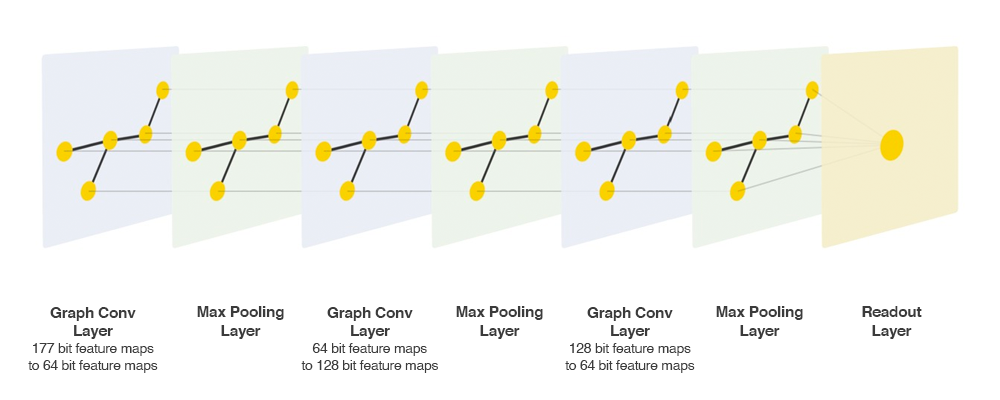
\includegraphics[width=1\linewidth]{img/gcn-layers.png}
		%   \captionof{figure}{Graph processing layers in our GCN implementation. The graph convolution layers apply operations on each individual node's feature maps based on neighbouring nodes. A ReLU function activates the output from each convolutional layer. A TanH function activates the final readout layer.}
		%  \label{fig:dvgcnarchi2}
		% \end{minipage}
	% }
